\documentclass[t,usenames,dvipsnames]{beamer}
\usetheme{Copenhagen}
\setbeamertemplate{headline}{} % remove toc from headers
\beamertemplatenavigationsymbolsempty

\usepackage{amsmath, xcolor, tikz, pgfplots, array, tcolorbox, colortbl, bm}

\pgfplotsset{compat = newest}
\usetikzlibrary{arrows.meta, calc, decorations.pathreplacing}
\pgfplotsset{every axis/.append style = {axis lines = middle}}
\pgfplotsset{every tick label/.append style={font=\scriptsize}}
\everymath{\displaystyle}

\tikzstyle{input} = [circle, text centered, radius = 1cm, draw = black]
\tikzstyle{function} = [rectangle, text centered, minimum width = 2cm, minimum height = 1cm, draw = black]

\title{Inverse Functions}
\author{}
\date{}

\AtBeginSection[]
{
  \begin{frame}
    \frametitle{Objectives}
    \tableofcontents[currentsection]
  \end{frame}
}

\begin{document}

\begin{frame}
    \maketitle
\end{frame}

\begin{frame}{Intro}
An inverse function works like an ``undo" function. \newline\\ \pause

If we give a function input it gives us output in return. \newline\\ \pause 

If we want our original input back, we can give our output to the inverse function and get our original input back.
\end{frame}

\begin{frame}{Visual Interpretation}
Original Function $f(x) = x^2$ \qquad Inverse Function: $g(x) = \sqrt{x}$ \newline\\
\begin{center}
    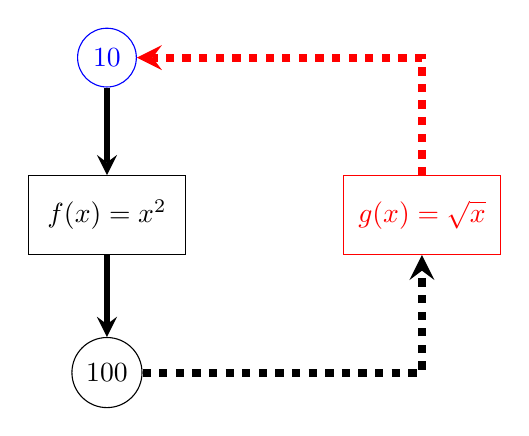
\begin{tikzpicture}[node distance = 2cm]
\node (inputVal) [input, color=blue] {\color{blue}10};
\node (func) [function, below of = inputVal] {$f(x)=x^2$};
\node (outputVal) [input, below of = func] {100};
\node (invFunc) [function, right of = func, xshift = 2cm, color=red] {\color{red}$g(x)=\sqrt{x}$};

\draw [->, >=stealth, thick, line width = 0.75mm] (inputVal) -- (func);
\draw [->, >=stealth, thick, line width = 0.75mm] (func) -- (outputVal);
\draw [->, >=stealth, thick, dashed, line width = 1mm] (outputVal) -| (invFunc);
\draw [->, >=stealth, thick, dashed, line width = 1mm, color = red] (invFunc) |- (inputVal);
\end{tikzpicture}
\end{center}
\end{frame}

\begin{frame}{Mathematical Definition of Inverse Functions}
Mathematically, two functions $f(x)$ and $g(x)$ are inverses of each other if {\color{blue}\textbf{both}} of the following are true: \newline\\   \pause

\begin{itemize}
    \item $(g \circ f)(x) = x$ for all $x$ in the domain of $f$ \newline\\  \pause
    \item $(f \circ g)(x) = x$ for all $x$ in the domain of $g$   
\end{itemize}
\end{frame}


\section{Determine if a relation or function has an inverse}

\begin{frame}{Horizontal Line Test}
When we first looked at relations, we knew they were functions if they passed the \alert{Vertical Line Test}. \newline\\ \pause

For a function to have an inverse that is also a function, it must pass a similar test known as the {\color{blue}\textbf{Horizontal Line Test}}.    \newline\\  \pause

\begin{tcolorbox}[colframe=green!60!black, title=Horizontal Line Test]{If each horizontal line intersects the graph \textbf{\underline{at most once}}, then the function has an inverse.} 
\end{tcolorbox}
\pause

\emph{Note:} A function that passes the Horizontal Line Test is also said to be \alert{invertible} or \alert{one-to-one}.
\end{frame}

\begin{frame}{Example 1}
Determine if the following relations or functions have an inverse.   \newline\\
(a) \quad $F = \{(-1,1), \, (0,2), \, (2,1) \}$ \newline\\  
\begin{minipage}{0.55\textwidth}
\onslide<2->{
\begin{tikzpicture}[scale=0.8]
\begin{axis}[
xmin = -3, xmax = 3,
ymin = 0, ymax = 3
]
\addplot [color=blue, mark=*, only marks] coordinates {(-1,1) (0,2) (2,1)};
\only<3->{\addplot[color=red, dashed, thick, domain=-3:3] {1};}
\end{axis}
\end{tikzpicture}}
\end{minipage}
\begin{minipage}{0.4\textwidth}
\onslide<4->{Does not have an inverse.}
\end{minipage}
\end{frame}

\begin{frame}{Example 1}
(b) \quad $f(x) = \frac{1-2x}{5}$   \newline\\ \bigskip
\begin{minipage}{0.55\textwidth}
\onslide<2->{
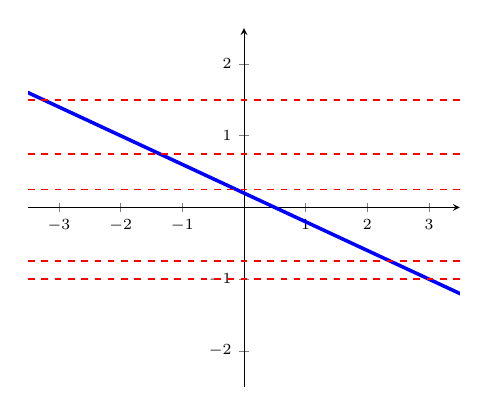
\begin{tikzpicture}[scale=0.8]
\begin{axis}[
xmin = -3.5, xmax = 3.5,
ymin = -2.5, ymax = 2.5
]
\addplot[color=blue, ultra thick] {-0.4*x+0.2};
\only<3->{
\addplot[color=red, dashed, thick, domain=-3.5:3.5] {1.5};
\addplot[color=red, dashed, thick, domain=-3.5:3.5] {0.75};
\addplot[color=red, dashed, thick, domain=-3.5:3.5] {0.25};
\addplot[color=red, dashed, thick, domain=-3.5:3.5] {-0.75};
\addplot[color=red, dashed, thick, domain=-3.5:3.5] {-1};
}
\end{axis}
\end{tikzpicture}}
\end{minipage}
\begin{minipage}{0.4\textwidth}
\onslide<4->{Has an inverse.}
\end{minipage}
\end{frame}

\begin{frame}{Example 1}
(c) \quad $g(x) = \frac{2x}{1-x}$ \newline\\    \bigskip
\begin{minipage}{0.55\textwidth}
\onslide<2->{
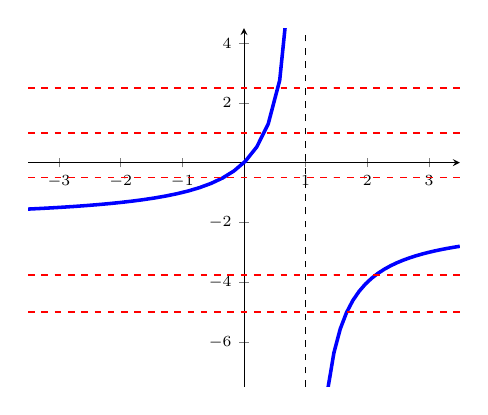
\begin{tikzpicture}[scale=0.8]
\begin{axis}[
xmin = -3.5, xmax = 3.5,
ymin = -7.5, ymax = 4.5
]
\addplot[color=blue, ultra thick, domain=-3.5:0.95] {(2*x)/(1-x)};
\addplot[color=blue, ultra thick, domain=1.05:3.5] {(2*x)/(1-x)};
\draw[dashed] (axis cs: 1,-7.5) -- (axis cs: 1,4.5);
\only<3->{
\addplot[color=red, dashed, thick, domain=-3.5:3.5] {2.5};
\addplot[color=red, dashed, thick, domain=-3.5:3.5] {1};
\addplot[color=red, dashed, thick, domain=-3.5:3.5] {-0.5};
\addplot[color=red, dashed, thick, domain=-3.5:3.5] {-3.75};
\addplot[color=red, dashed, thick, domain=-3.5:3.5] {-5};
}
\end{axis}
\end{tikzpicture}}
\end{minipage}
\begin{minipage}{0.4\textwidth}
\onslide<4->{Has an inverse.}
\end{minipage}
\end{frame}

\begin{frame}{Example 1}
(d) \quad $h(x) = x^2 - 2x + 4$ \newline\\  \bigskip
\begin{minipage}{0.55\textwidth}
\onslide<2->{
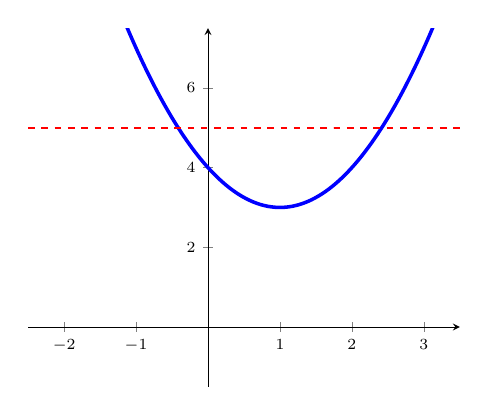
\begin{tikzpicture}[scale=0.8]
\begin{axis}[
xmin = -2.5, xmax = 3.5,
ymin = -1.5, ymax = 7.5
]
\addplot[color=blue, ultra thick, samples=200, smooth] {x^2 - 2*x + 4};
\only<3->{\addplot[color=red, dashed, thick, domain=-2.5:3.5] {5};}
\end{axis}
\end{tikzpicture}}
\end{minipage}
\begin{minipage}{0.4\textwidth}
\onslide<4->{Does not have an inverse.}
\end{minipage}
\end{frame}

\section{Find the inverse of a function}

\begin{frame}{Inverse Function Notation}
For a given function $f(x)$, the notation for the inverse of $f(x)$ is
\[ f^{-1}(x) \]
\end{frame}

\begin{frame}[c]{How to Find the Inverse of a Function}
\begin{enumerate}
    \item Write as $y = f(x)$   \newline\\ \pause
    \item Switch the $x$ and $y$ \newline\\ \pause 
    \item Solve for $y$ and write using inverse notation $f^{-1}(x)$.
\end{enumerate}
\end{frame}

\begin{frame}{Example 2}
Find the inverse of each.   \newline\\
(a) \quad $f(x) = \frac{1-2x}{5}$ 
\begin{align*}
    \onslide<2->{y &= \frac{1-2x}{5}} \\[8pt]
    \onslide<3->{x &= \frac{1-2{\color{red}y}}{5}} \\[8pt]
    \onslide<4->{5x &= 1-2{\color{red}y}} \\[6pt]
    \onslide<5->{-2{\color{red}y} &= 5x - 1} \\[6pt]
    \onslide<6->{{\color{red}y} &= \frac{5x-1}{-2}}
\end{align*}
\end{frame}

\begin{frame}[c]{Example 2}
    \[f^{-1}(x) = \frac{-5x+1}{2}\]
\end{frame}

\begin{frame}{Example 2}
(b) \quad $g(x) = \frac{2x}{1-x}$
\begin{align*}
    \onslide<2->{y &= \frac{2x}{1-x}} \\[8pt]
    \onslide<3->{x &= \frac{2{\color{red}y}}{1-{\color{red}y}}} \\[8pt]
    \onslide<4->{x(1-{\color{red}y}) &= 2{\color{red}y}} \\[6pt]
    \onslide<5->{x-x{\color{red}y} &= 2{\color{red}y}} \\[6pt]
    \onslide<6->{x &= 2{\color{red}y} + x{\color{red}y}} \\[6pt]
    \onslide<7->{x &= {\color{red}y}(2+x)}
\end{align*}
\end{frame}

\begin{frame}[c]{Example 2 \quad $g(x) = \tfrac{2x}{1-x}$}
\begin{align*}
    \frac{x}{2+x} &= {\color{red}y} \\[12pt]
    \onslide<2->{g^{-1}(x) &= \frac{x}{x+2}}
\end{align*}
\end{frame}

\begin{frame}{Example 2}
(c) \quad $h(x) = \sqrt{x+2} - 1$
\begin{align*}
    \onslide<2->{y &= \sqrt{x+2}-1} \\[6pt]
    \onslide<3->{x &= \sqrt{{\color{red}y}+2} - 1} \\[6pt]
    \onslide<4->{x+1 &= \sqrt{{\color{red}y}+2}} \\[6pt]
    \onslide<5->{(x+1)^2 &= {\color{red}y} + 2} \\[6pt]
    \onslide<6->{(x+1)^2 -2 &= {\color{red}y}} \\[10pt]
    \onslide<7->{h^{-1}(x) &= (x+1)^2 - 2}
\end{align*}
\end{frame}

\section{Find the domain and range of the inverse of a function}

\begin{frame}{Domain and Range of Inverse Functions}
In the previous example, we found the inverse of a function by switching the $x$ and the $y$ in the equation. \newline\\ \pause

By doing this, we also switch the \alert{domain and range} of the original function and its inverse. \newline\\ \pause

\begin{center}
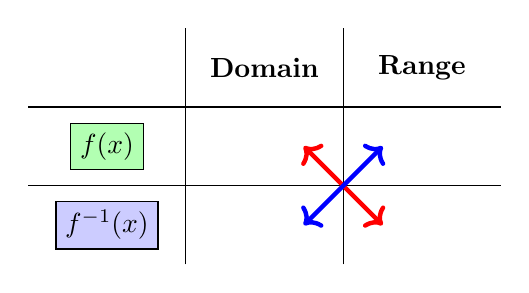
\begin{tikzpicture}
\node [rectangle, draw, fill=green!30] at (0,0.5) {$f(x)$};
\node [rectangle, draw, fill=blue!20] at (0,-0.5) {$f^{-1}(x)$};
\draw (1,-1) -- (1,2);  % creates 1st column
\draw (-1,1) -- (5,1);
\draw (3,-1) -- (3,2);  % creates 2nd column
\node at (2,1.5) {\textbf{Domain}};
\node at (4,1.5) {\textbf{Range}};
\draw (-1,0) -- (5,0);
\onslide<4->{\draw[<->, ultra thick, red] (2.5,0.5) -- (3.5,-0.5);}
\onslide<5->{\draw[<->, ultra thick, blue] (2.5,-0.5) -- (3.5,0.5);}
\end{tikzpicture}
\end{center}
\end{frame}

\begin{frame}{Visual Interpretation of Finding Inverse}
Switching the $x$ and $y$ variables when finding the inverse of a function involves \alert{reflecting the graph of the function along the line $y=x$}.   \pause

\begin{center}
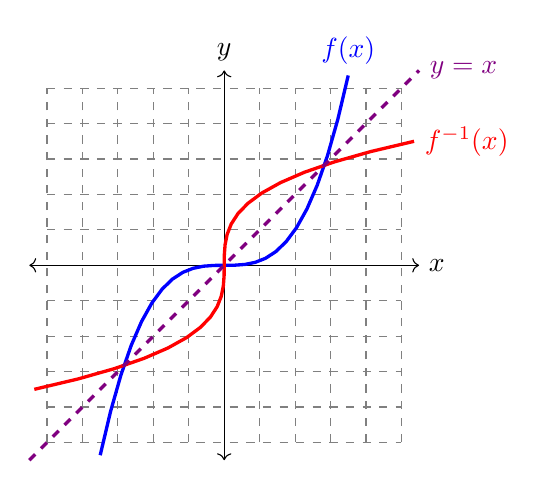
\begin{tikzpicture}[scale=0.45]
\draw [color=gray, dashed] (-5,-5) grid (5,5);
\draw[<->] (-5.5,0) -- (5.5,0) node [right] {$x$};
\draw[<->] (0,-5.5) -- (0,5.5) node [above] {$y$};
\draw [color=blue, very thick, domain=-1.75:1.75, xscale=2] plot (\x, {\x*\x*\x}) node [above] {$f(x)$};
\draw [color=red, very thick, domain=-1.75:1.75, yscale=2] plot ({\x*\x*\x}, \x) node [right] {$f^{-1}(x)$};
\draw [color=violet, very thick, dashed] (-5.5,-5.5) -- (5.5,5.5) node [right] {$y=x$};
\end{tikzpicture}
\end{center}
\end{frame}

\begin{frame}[c]{Domain and Range Restrictions}
Sometimes you have to restrict the domain of the function so that it is a reflection of its inverse across the line $y=x$
\end{frame}

\begin{frame}{Example 3}
Find the domain and range of the inverse of each. \newline\\
(a) \quad $f(x) = \frac{1-2x}{5}$
\onslide<2->{\quad $f^{-1}(x) = \frac{-5x+1}{2}$}   \\[10pt]
\begin{center}
\onslide<3->{
\setlength{\extrarowheight}{6pt}
\begin{tabular}{c|c|c}
                &  \textbf{Domain}  &   \textbf{Range}  \\      \hline
    $f(x)$      &  \onslide<4->{\cellcolor{yellow!75}$\bm{(-\infty,\infty)}$}  &  \onslide<6->{\cellcolor{green!60}$\bm{(-\infty,\infty)}$}                   \\[6pt] \hline
    $f^{-1}(x)$ & \onslide<7->{\cellcolor{green!60}$\bm{(-\infty,\infty)}$}  & \onslide<5->{\cellcolor{yellow!75}$\bm{(-\infty,\infty)}$}                  \\[6pt]
\end{tabular}}
\end{center}
\begin{align*}
\onslide<8->{\text{Domain of } f^{-1}(x): &\quad (-\infty, \infty)}    \newline\\
\onslide<9->{\text{Range of } f^{-1}(x): &\quad (-\infty, \infty)}
\end{align*}
\end{frame}

\begin{frame}{Example 3}
(b) \quad $g(x) = \frac{2x}{1-x}$
\onslide<2->{\quad $g^{-1}(x) = \frac{x}{x+2}$} \\[10pt]
\begin{center}
\onslide<3->{
\setlength{\extrarowheight}{6pt}
\begin{tabular}{c|c|c}
                &  \textbf{Domain}  &   \textbf{Range}  \\      \hline
    $g(x)$      &  \onslide<4->{\cellcolor{yellow!75}$\bm{x \neq 1}$}  &  \onslide<7->{\cellcolor{green!60}$\bm{y \neq -2}$}                   \\[6pt] \hline
    $g^{-1}(x)$ & \onslide<6->{\cellcolor{green!60}$\bm{x \neq -2}$}  & \onslide<5->{\cellcolor{yellow!75}$\bm{y \neq 1}$}                  \\[6pt]
\end{tabular}}
\end{center}
\begin{align*}
\onslide<8->{\text{Domain of } g^{-1}(x): &\quad (-\infty, -2) \cup (-2,\infty)}    \newline\\
\onslide<9->{\text{Range of } g^{-1}(x): &\quad (-\infty, 1) \cup (1,\infty)}
\end{align*}
\end{frame}

\begin{frame}{Example 3}
(c) \quad $h(x) = \sqrt{x+2} - 1$
\onslide<2->{\quad $h^{-1}(x) = (x+1)^2 -2$} \\[10pt]
\begin{center}
\onslide<3->{
\setlength{\extrarowheight}{6pt}
\begin{tabular}{c|c|c}
                &  \textbf{Domain}  &   \textbf{Range}  \\      \hline
    $h(x)$      &  \onslide<4->{\cellcolor{yellow!75}$\bm{x \geq -2}$}  &  \onslide<6->{\cellcolor{green!60}$\bm{y \geq -1}$}                   \\[6pt] \hline
    $h^{-1}(x)$ & \onslide<7->{\cellcolor{green!60}$\bm{x \geq -1}$}  & \onslide<5->{\cellcolor{yellow!75}$\bm{y \geq -2}$}                  \\[6pt]
\end{tabular}}
\end{center}
\begin{align*}
\onslide<8->{\text{Domain of } h^{-1}(x): &\quad [-1, \infty)}    \newline\\
\onslide<9->{\text{Range of } h^{-1}(x): &\quad [-2, \infty)}
\end{align*}
\end{frame}

\begin{frame}{Example 3}
(d) \quad $j(x) = x^2 - 2x + 4, \quad x \leq 1$   \newline\\
\begin{center}
\onslide<2->{
\begin{tikzpicture}[scale=0.8]
\begin{axis}[
xmin=-2, xmax = 4,
ymin=0, ymax = 8
]
\addplot[color=blue, ultra thick, samples=200, smooth, domain=-1:1] {x^2-2*x+4};
\only<3->{\addplot[color=blue, ultra thick, samples=200, smooth, domain=-1:3] {x^2-2*x+4};}
\end{axis}
\end{tikzpicture}}
\end{center}
\end{frame}

\begin{frame}{Example 3}
(d) \quad $j(x) = x^2 - 2x + 4 \quad x \leq 1$
\begin{align*}
    \onslide<2->{y &= x^2 - 2x + 4} \\[6pt]
    \onslide<3->{x &= {\color{red}y}^2 - 2{\color{red}y} + 4} \\[6pt]
    \onslide<4->{x &= ({\color{red}y} - 1)^2+3} \\[6pt]
    \onslide<5->{x-3 &= ({\color{red}y} - 1)^2} \\[6pt]
    \onslide<6->{\pm \sqrt{x-3} &= {\color{red}y} - 1} \\[6pt]
    \onslide<7->{1\pm \sqrt{x-3} &= \color{red}y} \\[6pt]
    \onslide<8->{j^{-1}(x) &= 1 \pm \sqrt{x-3}} \\[6pt]
    \onslide<9->{j^{-1}(x) &= 1 - \sqrt{x-3}}
\end{align*}
\end{frame}

\begin{frame}{Example 3}
(d) \quad $j(x) = x^2 - 2x + 4 \quad x \leq 1 \qquad j^{-1}(x) = 1 - \sqrt{x-3}$ \newline\\ 
\begin{center}
\onslide<2->{
\setlength{\extrarowheight}{5pt}
\begin{tabular}{c|c|c}
                &   \textbf{Domain}             &   \textbf{Range}              \\ \hline 
    $j(x)$      & \onslide<3->{\cellcolor{yellow!75}$\bm{x \leq 1}$}      & \onslide<6->{\cellcolor{green!60}$\bm{y \geq 3}$}      \\[5pt] \hline
    $j^{-1}(x)$ & \onslide<5->{\cellcolor{green!60}$\bm{x \geq 3}$}      & \onslide<4->{\cellcolor{yellow!75}$\bm{y \leq 1}$}      \\[5pt]
\end{tabular}}
\end{center}
\begin{align*}
    \onslide<7->{\text{Domain of $j^{-1}(x)$:} \quad& [3, \infty)} \newline\\ 
    \onslide<8->{\text{Range of $j^{-1}(x)$:} \quad& (-\infty, 1]}
\end{align*}
\end{frame}

\end{document}
